\Chapter{Megvalósítás}

%%%%%%%%%%%%%%%%%%%%%%%%%%%%%%%%%%%%%%%%%%%%%%%%%%%%%%%%%%%%%%%%%%%%%%%%%%%%%%%%%%%%%%%%%%%%%%%%%%%%%%%%%
%%%%%%%%%%%%%%%%%%%%%%%%%%%%%%%%%%%%%%%%%%%%%%%%% 4 . 1 %%%%%%%%%%%%%%%%%%%%%%%%%%%%%%%%%%%%%%%%%%%%%%%%%
%%%%%%%%%%%%%%%%%%%%%%%%%%%%%%%%%%%%%%%%%%%%%%%%%%%%%%%%%%%%%%%%%%%%%%%%%%%%%%%%%%%%%%%%%%%%%%%%%%%%%%%%%

\section{Előkészületek}

\subsection{Visual Studio Code}

Első lépésben szükségünk van egy olyan fejlesztőkörnyezetre, mely rendelkezik terminállal. Választásom a \textit{Visual Studio Code} nevű környezetre esett. Egyszerű, segítőkész, könnyen átlátható fejlesztőkörnyezetről beszélünk, mely számos programozási nyelvet támogat, illetve segítséget nyújt használatukkor (\ref{fig:vscode}. ábra).

\begin{figure}[h]
	\centering
		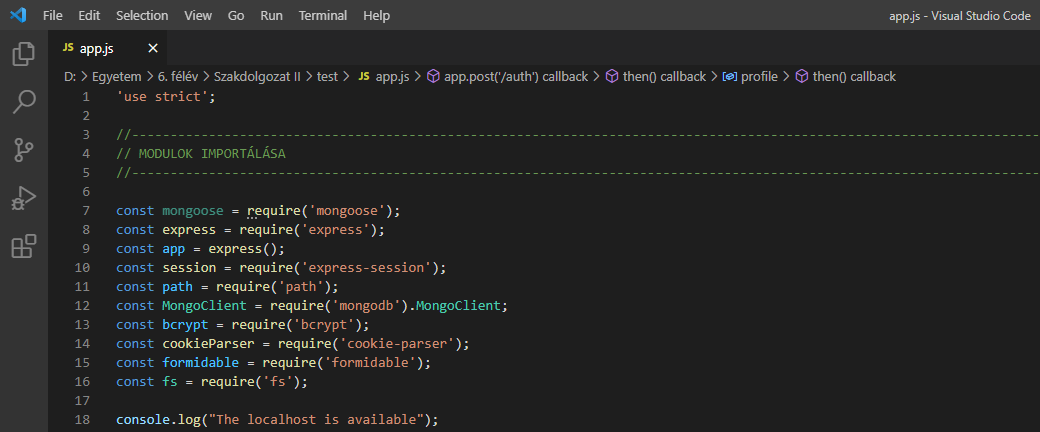
\includegraphics[width=15truecm, height=7truecm]{images/vscode.png}
	\caption{A Visual Studio Code felülete}
	\label{fig:vscode}
\end{figure}

\subsection{Node.js}

Az előző fejezetben összehasonlításra került néhány potenciális rendszer, jómagam pedig a \textit{Node.js} mellett döntöttem. Következő lépésben üzembe kell helyeznünk az említett keretrendszert, melyben a programot írjuk. A rendszert a hivatalos weboldaláról érhetjük el. Letöltés és telepítés után rendelkezésünkre is áll a szoftver. Első lépésben konfigurálnunk kell a program "szívét", a \textit{package.json} fájlt. Ez tartalmazza a fontos metaadatokat a projektünkhöz (például a program belépési pontját), ezek közül is kiemelve a "függőségeket" (dependency-ket). A függőségek azt jelölik, hogy milyen modulokra (és azok mely verzióira) van szükség a program teljesértékű futtatásához. A \textit{package.json} konfigurálásához az alábbi parancsot kell begépelnünk:

\begin{verbatim}
$ npm init
\end{verbatim}

A folyamaton belül, pár további változó megadása után már ténylegesen készen áll a projektünk.

Előreláthatólag szükségünk lesz modulokra, így (a megfelelő mappába való elnavigálás után) a következő parancsot kell begépelnünk a terminálba:

\begin{verbatim}
$ npm install <modulnev>
\end{verbatim}

Telepítés után a függőség bekerül a \textit{package.json} fájlba, így a rendszer tudni fogja, hogy a megadott modult telepíteni kell használat előtt (abba az esetben, ha például más mappából futtatjuk a projektet).

Ha minden készen áll a használatra, akkor a lentebb látható paranccsal futtathatjuk a programunkat:

\begin{verbatim}
$ node <fajl.kiterjesztes>
\end{verbatim}

Ezzel készen is vagyunk a Node.js telepítésével, viszont még szükségünk lesz további előkészületekre.

\subsection{MongoDB}

Ahogyan webes keretrendszert, úgy adatbázist is választani kell. A választásom pedig a \textit{MongoDB}-re esett, mégpedig azért, mert számos különböző típusú adattal dolgozunk, melyeket nem feltétlenül lehet struktúrába rendezni. Az összehasonlításoknál láthattuk, hogy sémakötöttség szempontjából a NoSQL adatbázisok rugalmasabbak az SQL alapúaknál, ezért a MongoDB kézenfekvő megoldás.

Ahogy a Node.js-t, úgy a MongoDB-t is a hivatalos weboldaláról érhetjük el. Ebben az esetben is telepítésre, valamint installációra lesz szükség. Telepítés után pedig csatlakoznunk kell az adott adatbázishoz. Ezt elősegítendő, a program rendelkezik egy saját parancssoros felülettel. Itt az alábbi parancsot kell megadnunk:

\begin{verbatim}
$ mongod
\end{verbatim}

Ennek hatására a konfigurációs fájl (\textit{mongo.cfg}) alapján csatlakozik az adatbázishoz, így a Node.js-ből is hozzáférhetünk a csatlakoztatott adatbázishoz, és annak tartalmához (például a kollekciókhoz).

\subsection{Egyéb potenciálisan hasznos programok}

\noindent{\textbf{\large{Postman}}}\\

Említést érdemel egy további alkalmazás, mely nagy segítséget nyújt az applikációnk tesztelésében. Ez pedig nem más, mint a \textit{Postman}. Ez az asztali alkalmazás képes - többek között - felhasználói adatbevitelt szimulálni, így tesztelhetjük a webapplikációnkat különböző kérések elküldésével (\ref{fig:postman}. ábra).

\newpage

\begin{figure}[h]
	\centering
		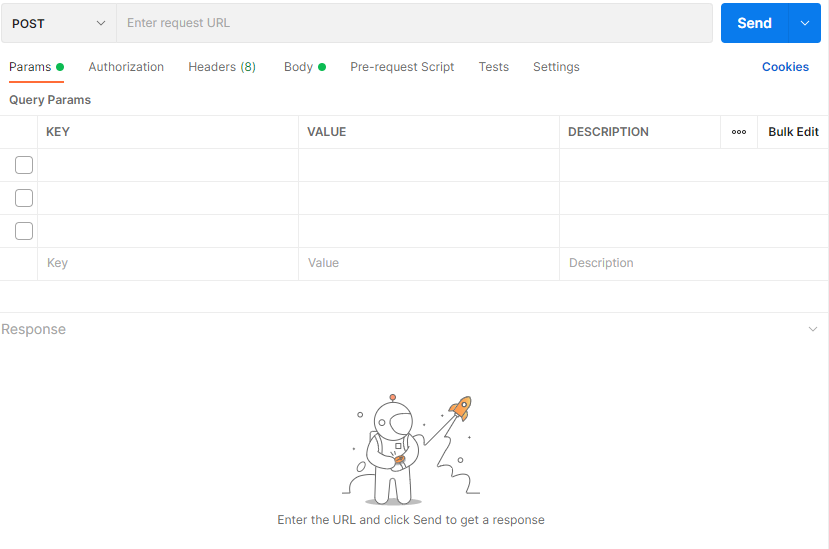
\includegraphics[width=15truecm, height=9truecm]{images/postman.png}
	\caption{A Postman grafikus felülete}
	\label{fig:postman}
\end{figure}

Például bejelentkezési folyamatot így futtathatunk:

\begin{enumerate}
\item{Be kell írnunk az URL-t, melyre tesztelni szeretnénk, valamint a kérés típusát (\texttt{get} és \texttt{post} típusokat különböztetünk itt meg, mivel ez a két leggyakrabban alkalmazott metódus).}
\item{Meg kell adnunk a küldendő adatokat. Ezek elég változatosak lehetnek, leggyakrabban \texttt{header} és \texttt{body} paramétereket és értékeiket adunk át.}
\item{Végül pedig a "\textit{Küldés}" gombbal elküldjük a kérést a megadott szerverre.}
\end{enumerate}

Küldés után a válaszablakban találhatjuk a kérés eredményeit. Itt láthatjuk például a HTTP válasz státuszkódját, a futás idejét miliszekundumokban, viszont a legfontosabb a válaszkód, melyet akár többféle nyelven tudjuk megjeleníteni. E kód segítségével tudjuk ellenőrizni azt, hogy valóban helyesen működik-e a programunk.\\

\noindent{\textbf{\large{MongoDB Atlas}}}\\

Említésre került, hogy a MongoDB applikációja alapvetően parancssoros felületű. Ennek értelmében a csatlakoztatott adatbázist és annak tartalmát (például a kollekcióit) szintén parancssoros felületen keresztül érhetjük el. Amennyiben viszont igényünk van rá, megtehetjük mindezt grafikus felületen is. Ezt a \textit{MongoDB Atlas} nevű webalkalmazás teszi lehetővé (\ref{fig:atlas}. ábra). További előnyeként meg kell említenünk, hogy a MongoDB Atlas segítségével felhőszolgáltatásként használhatjuk adatbázisunkat, így az adataink nem lokálisan, hanem felhőben tárolódnak.

\newpage

\begin{figure}[h]
	\centering
		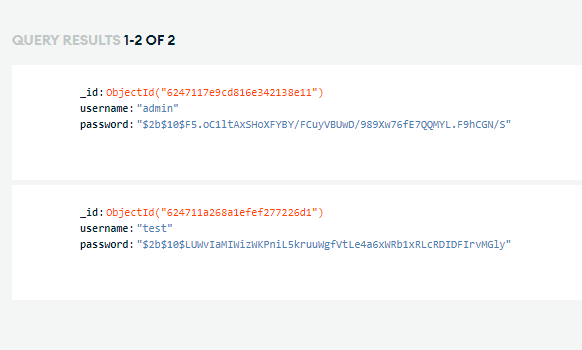
\includegraphics[width=12truecm, height=7truecm]{images/atlas.png}
	\caption{A MongoDB Atlas felülete}
	\label{fig:atlas}
\end{figure}

%%%%%%%%%%%%%%%%%%%%%%%%%%%%%%%%%%%%%%%%%%%%%%%%%%%%%%%%%%%%%%%%%%%%%%%%%%%%%%%%%%%%%%%%%%%%%%%%%%%%%%%%%
%%%%%%%%%%%%%%%%%%%%%%%%%%%%%%%%%%%%%%%%%%%%%%%%% 4 . 2 %%%%%%%%%%%%%%%%%%%%%%%%%%%%%%%%%%%%%%%%%%%%%%%%%
%%%%%%%%%%%%%%%%%%%%%%%%%%%%%%%%%%%%%%%%%%%%%%%%%%%%%%%%%%%%%%%%%%%%%%%%%%%%%%%%%%%%%%%%%%%%%%%%%%%%%%%%%

\section{A program általános jellemzői}

A weboldalak mind HTML nyelvben íródnak, viszont \textit{.ejs} kiterjesztésűek. Ennek az az oka, hogy egy bizonyos \textit{EJS view engine}-t alkalmazunk. Ennek okát a későbbiekben kifejtjük. A weboldalak stílusát CSS stíluslapokkal írjuk meg. Külön témát alkotunk a bejelentkezési oldalra (kék), a felhasználói-, adminisztrátori felületekre, illetve a sikeres műveletet értesítő oldalakra (zöld), valamint a hibajelző oldalakra (piros).

A továbbiakban fontos megjegyezni, hogy az átirányításokat \textit{Express} rendszerrel hajtjuk végre. Szándékosan nem modulként hivatkozunk rá, hiszen ez egy, a Node.js számára fejlesztett backend keretrendszer, mely nagyban megkönnyíti a webapplikációk fejlesztésének menetét. Telepíteni viszont modulként kell:

\begin{verbatim}
$ npm install express
\end{verbatim}

Ahogyan már említettük, az Express végzi az átirányításokat (is). Például:

\begin{javascript}
app.get('/invalid', function(req, res) {
  res.render("invalid");
});
\end{javascript}

Ebben a példában a "\textit{/invalid}" nevű oldalra navigálás esetén az "\textit{invalid}" nevű fájlt tölti be a rendszer. Itt viszont vissza kell térnünk a .ejs kiterjesztésre. Ugyanis az Express HTML oldalakat nem tud betölteni. Emiatt kell használnunk az EJS-t, amely viszont megköveteli, hogy \textit{.html} helyett \textit{.ejs} legyen az oldalak kiterjesztése. Ez lényegében semmilyen változtatással nem jár, szintaktikájuk (ebben az esetben teljesen) megegyezik.

Szóba került a munkamenet-menedzselés is. Ezt az Express egyik alrendszerével, az \textit{Express-session}-nel, valamint a \textit{Cookie-parser} nevű modullal oldjuk meg. Míg az előbbi magát a munkamenetet kezeli, az utóbbi segítségével tudjuk módosítani a sütiket (példának okáért a sütik elévülési idejét - ez határozza meg a munkamenet hosszát, mely esetünkben 30 perc).

A projekten belüli navigációt, illetve útvonalkezelést a \textit{Path} nevű modullal végezzük. E modul képes többek között fájlok kiterjesztését, kiterjesztés nélküli nevét ("basename") lekérdezni, útvonalak abszolút voltát, vagy akár két útvonal közti relatív útvonalat is képes meghatározni. Nekünk a \texttt{resolve()} függvény lesz segítségünkre, mellyel az argumentumként megadott útvonalat és más mappákat lehet abszolút útvonalként beállítani. Emellett a \texttt{join()} metódus is hasznunkra lesz, mivel ezzel útvonalakat lehet összevonni. Továbbá egy bizonyos \texttt{\_\_dirname} változót is biztosít számunkra a modul, mely a futtatás helyét tárolja (mindig azt az útvonalat veszi fel értékként, amelyből futtattuk a programot).

Igényt tartunk még a \textit{Formidable} modulra is. Ez lehetővé teszi számunkra, hogy bejövő (felhasználó által elküldött, így rendelkezésünkre bocsátott), főleg fájlfeltöltési űrlapokat kezeljünk. Leglényegesebb funkciója a \texttt{parse()} függvény. Ezzel tudjuk a kapott űrlapot értelmezni, mind a kiválasztott fájl(ok), mind a hozzá kapcsolódó mezők szempontjából.

Végül pedig beimportáljuk az \textit{fs} nevű modult. Ezen modullal fájlműveleteket végezhetünk, például:
\begin{itemize}
\item{Fájl létrehozása}
\item{Fájl létezésének ellenőrzése}
\item{Fájl módosítása}
\item{Fájl törlése}
\item{Fájl átnevezése}
\end{itemize}
Számunkra a fájlfeltöltés folyamatában lesz hasznos. Erre a feltöltés részletezésénél térünk vissza.

%%%%%%%%%%%%%%%%%%%%%%%%%%%%%%%%%%%%%%%%%%%%%%%%%%%%%%%%%%%%%%%%%%%%%%%%%%%%%%%%%%%%%%%%%%%%%%%%%%%%%%%%%
%%%%%%%%%%%%%%%%%%%%%%%%%%%%%%%%%%%%%%%%%%%%%%%%% 4 . 3 %%%%%%%%%%%%%%%%%%%%%%%%%%%%%%%%%%%%%%%%%%%%%%%%%
%%%%%%%%%%%%%%%%%%%%%%%%%%%%%%%%%%%%%%%%%%%%%%%%%%%%%%%%%%%%%%%%%%%%%%%%%%%%%%%%%%%%%%%%%%%%%%%%%%%%%%%%%

\section{A program felépítése}

%%%%%%%%%%%%%%%%%%%%%%%%%%%%%%%%%%%%%%%%%%%%%%% 4 . 3 . 1 %%%%%%%%%%%%%%%%%%%%%%%%%%%%%%%%%%%%%%%%%%%%%%%

\subsection{A szerver konfigurációja}

Az applikációnk forráskódja elején a modulok importálása található. Ezután a szerver konfigurációja következik.

Első körben definiáljuk a munkamenethez szükséges paramétereket az Express-session segítségével:
\begin{itemize}
\item{\textbf{secret}: A munkamenet egyedi azonosító kulcsa. Ez általában egy bonyolult, véletlenszerűen generált string, melyet nem szabad nyilvánosságra hozni.}
\item{\textbf{saveUninitialized}: Egy boolean (logikai) típusú változó, mely jelzi, hogy az \textit{uninitialized} (létrehozott, de értékeket nem hordozó) munkamenetek mentésre kerüljenek-e, vagy sem.}
\item{\textbf{resave}: Szintén egy logikai értéket hordoz. Ez határozza meg, hogy mi történjen akkor, ha egy kérés során nem módosul a munkamenet. \texttt{True} érték esetén mentésre kerül, \texttt{false} esetén viszont nem. Versengéses kérések esetén (például amikor a felhasználó több párhuzamos kérést küld a szerver felé) a \textit{false} a jobb választás.}
\item{\textbf{cookie}: Itt tudjuk módosítani a sütik változóit. Mi csak egyetlen változót állítunk be, a \texttt{maxAge}-et. Ez határozza meg a süti (ezzel együtt a munkamenet) lejáratát. A mi esetünkben ez az érték fél óra.}
\end{itemize}

\noindent
A következő lépésben az Express működését szabályozzuk.

Az Express \texttt{json()} metódusa egy úgynevezett "middleware" metódus, melynek segítségével JSON-ként tudjuk értelmezni a bejövő kéréseket. Ennek a funkciónak köszönhető többek között az is, hogy a \texttt{req} változót és annak paramétereit használni tudjuk.

A következő metódus, melyet igénybe veszünk, a \texttt{urlencoded()}. Ez szintén egy middleware funkció, mely meghatározza, hogy csak UTF-8 kódolású oldalakat értelmezünk.

Ezután a \texttt{static()} függvényt hívjuk meg. Ezzel határozzuk meg, hogy melyik mappából töltsük be a futáshoz szükséges eszközöket (ebben az esetben, az EJS-eket, a stílusokat, valamint a letölthető tartalmat).

Következik az átirányítást kezelő motor konfigurációja. Ezt az Express \texttt{set()} metódusával tudjuk beállítani. A konfiguráció két fontos lépést foglal magában:
\begin{itemize}
\item{Beállítjuk a \texttt{view engine} paramétert. Mi az EJS-t használjuk, így az értékét erre állítjuk.}
\item{Majd pedig meghatározzuk a \texttt{view} változót, ennek értékét az EJS fájlok főmappájában határozzuk meg}
\end{itemize}

Utolsó változtatásként pedig meghívjuk a Cookie-parser modult.

%%%%%%%%%%%%%%%%%%%%%%%%%%%%%%%%%%%%%%%%%%%%%%% 4 . 3 . 2 %%%%%%%%%%%%%%%%%%%%%%%%%%%%%%%%%%%%%%%%%%%%%%%

\subsection{Autentikáció}

A program következő részében az autentikációval foglalkozunk. Ez egy \texttt{post} kérés, mely azt jelenti, hogy adatot küldünk a szervernek, mivel új adatot szeretnénk feltölteni, vagy meglévőt szeretnénk módosítani. Itt a bevitt adat hosszára, illetve típusára vonatkozó megkötések nincsenek. Az URL-ben nem jelenik meg a küldött adat, ezáltal a böngésző előzményei közt sem tárolódik. Az előző tények miatt érzékeny (fontos/titkos) adatokat érdemesebb post metódussal küldeni. Ennek értelmében tehát az autentikációt is post metódussal kezeljük.

A \textit{login.ejs} fájlban létrehozzuk a bejelentkezési űrlapot, melynek \texttt{action} paraméterét \textit{post}-ra állítjuk, így jelezve azt, hogy az űrlap post metódussal kerül küldésre. Az űrlap két \texttt{<input>} mezőből áll, egy a felhasználónak, egy a jelszónak,  előbbi \texttt{text}, utóbbi \texttt{password} típusú. A text mezőben minden karakter megjelenik, míg a jelszó mezőben csillagok jelennek meg, a titkosítást elősegítendő. Az űrlaphoz tartozik még a \textit{Bejelentkezés} gomb is, mellyel az űrlap tartalma elküldhető.

Az elküldött űrlapot az applikációnkban kezeljük. Először is bekérjük a felhasználó által bevitt adatokat, a nevet és a jelszót. Kiíratjuk a konzolra a felhasználói adatokat, majd csatlakozunk az adatbázishoz, ahol első körben rákeresünk a felhasználónévre. Abban az esetben, ha nem létezik, hibaüzenetet küldünk. Ha mégis létezik, a bcrypt modul segítségével összehasonlítjuk a begépelt jelszót az adatbázisban szereplő, kódolt jelszóval. Magától értetődő, hogy abban az esetben, ha nem egyeznek, szintén hibaüzenetet küldünk a felhasználónak. Egyezőség esetén viszont eltároljuk a munkamenet adatait (például a felhasználónevet), a Cookie-parser modul legenerálja a felhasználóhoz tartozó süti-adatokat (így a nagy jelentősséggel bíró lejárati dátumot is), végül pedig átirányít a megfelelő oldalra (a "nem-admin" felhasználókat a főoldalra, az adminisztrátort pedig a felhasználó hozzáadása oldalra.

Az autentikációt modellezi az alábbi folyamatábra (\ref{fig:autentikacio}. ábra):

\begin{figure}[h]
	\centering
		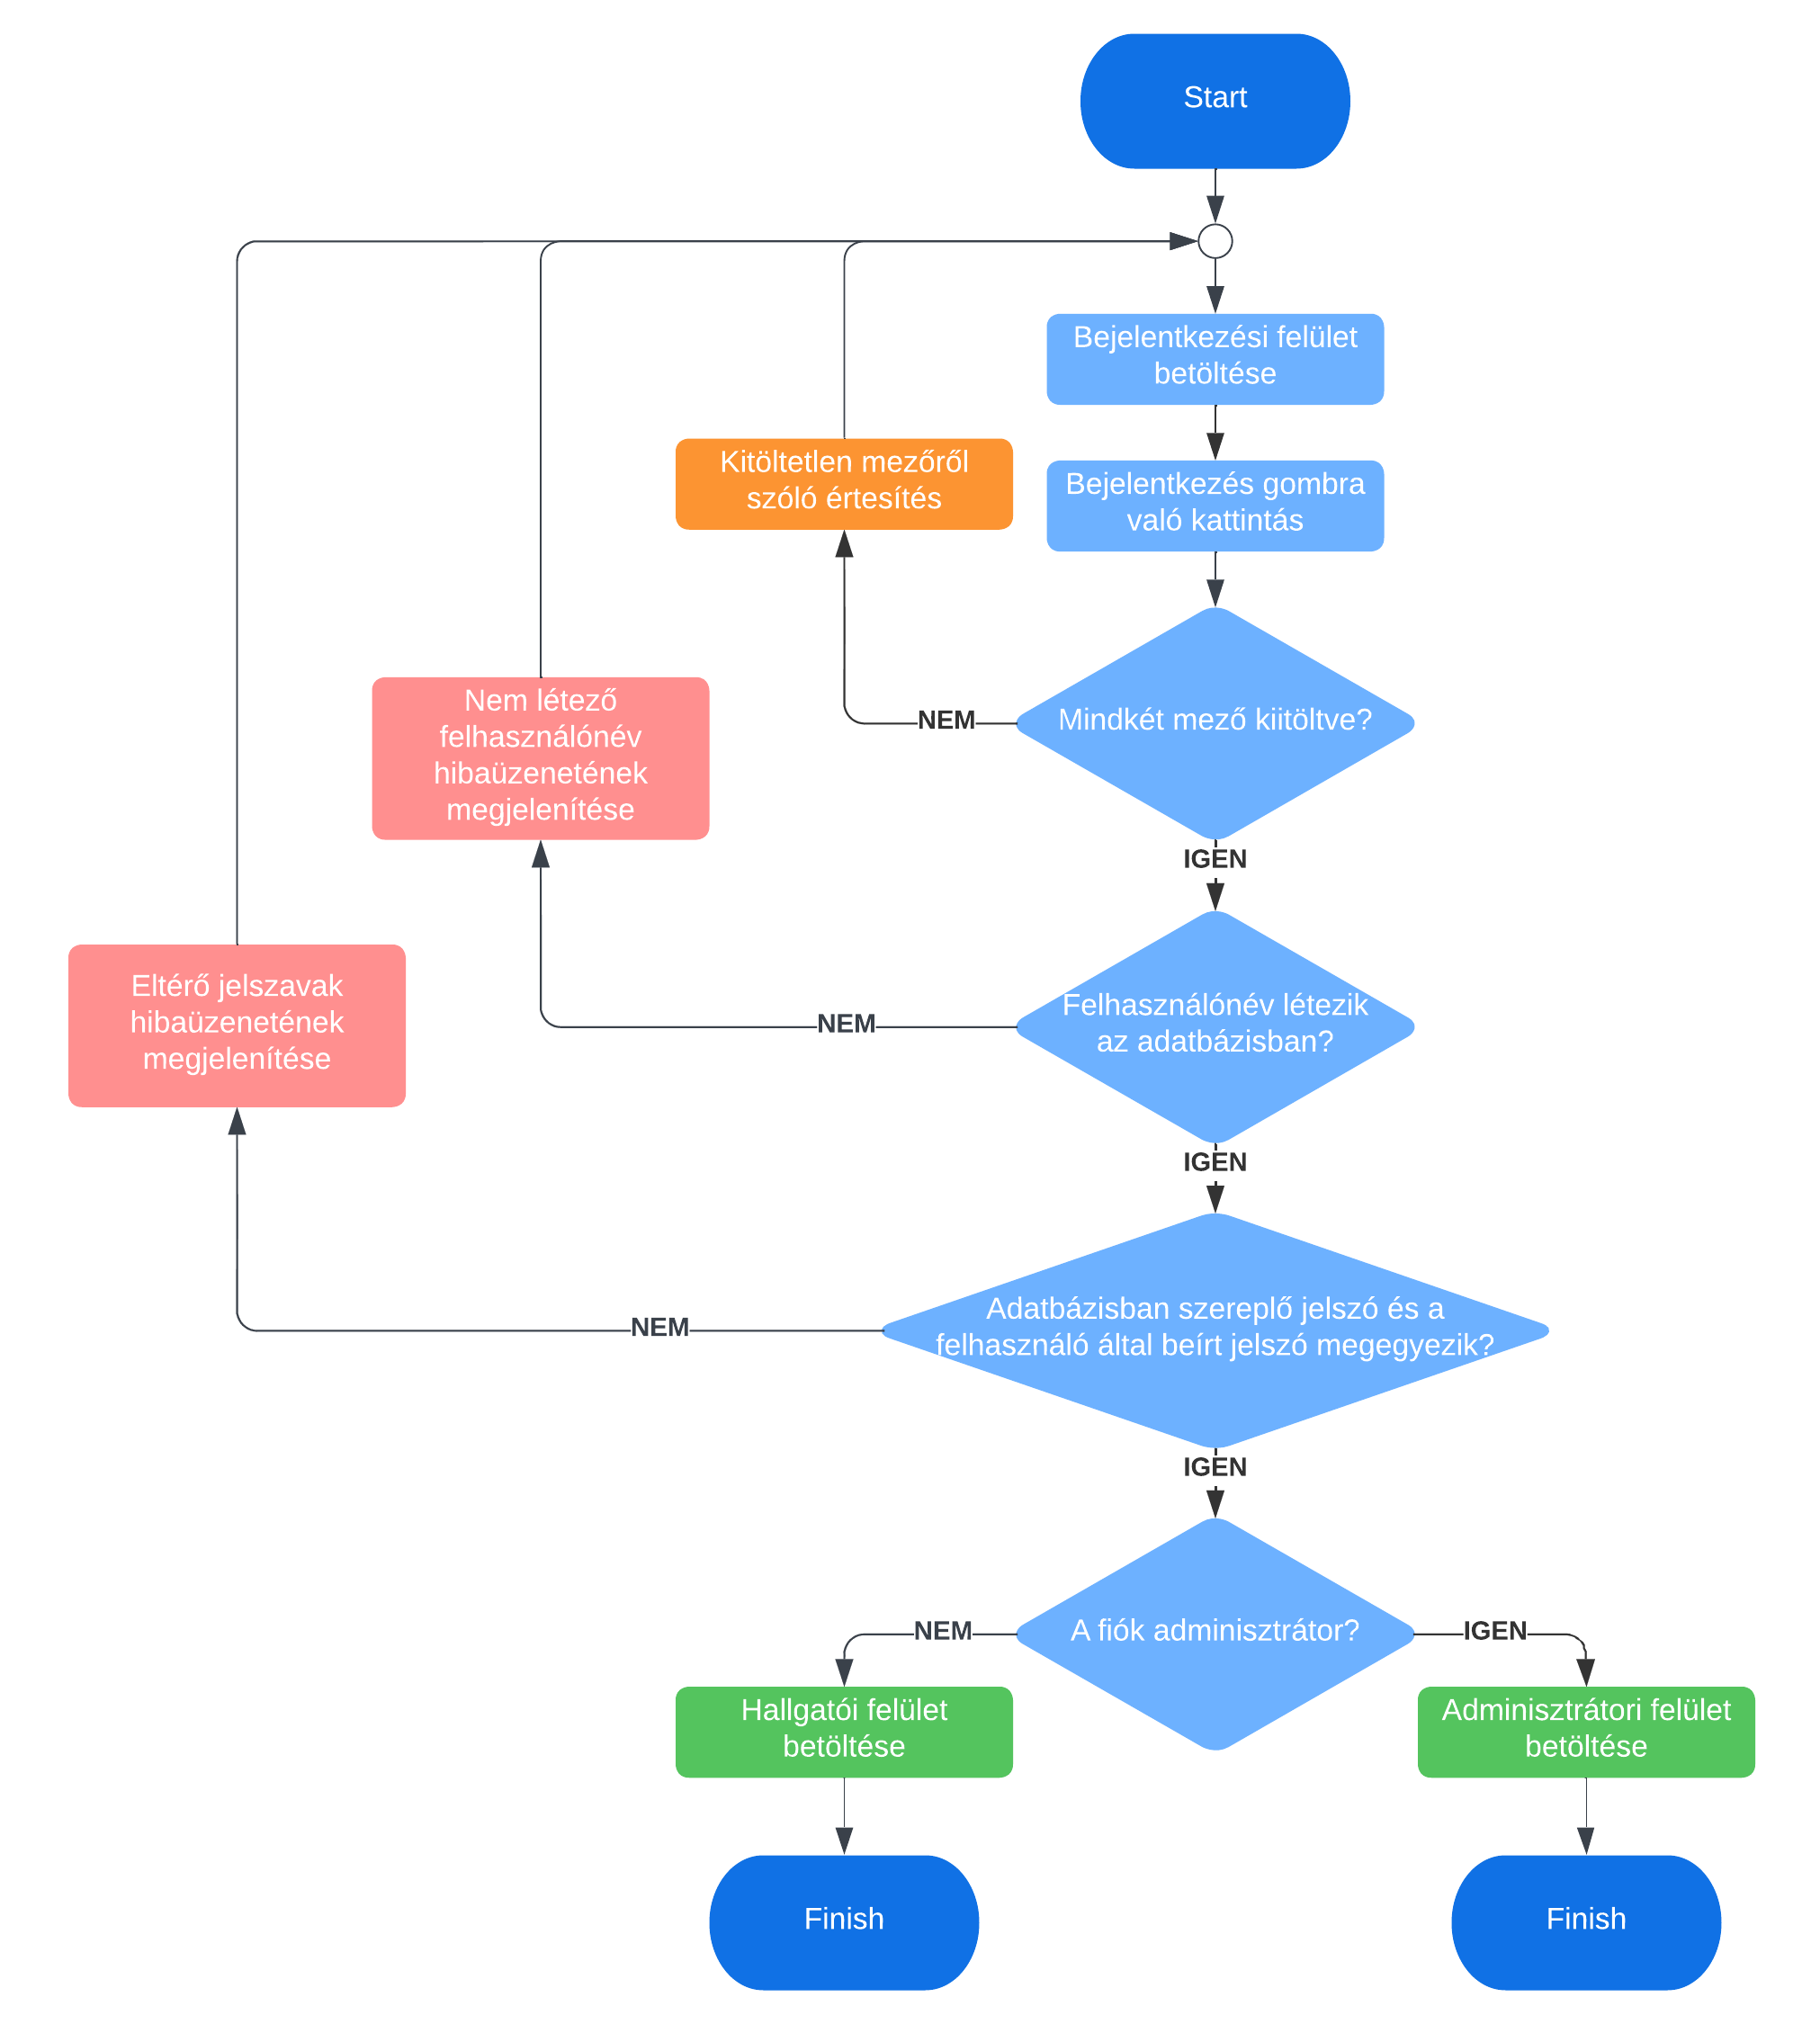
\includegraphics[width=15truecm, height=17truecm]{images/autentikacio.png}
	\caption{Az autentikáció folyamatábrája}
	\label{fig:autentikacio}
\end{figure}

%%%%%%%%%%%%%%%%%%%%%%%%%%%%%%%%%%%%%%%%%%%%%%% 4 . 3 . 3 %%%%%%%%%%%%%%%%%%%%%%%%%%%%%%%%%%%%%%%%%%%%%%%

\subsection{Adminisztrátori műveletek}

Következőleg az adminisztrátori műveletek kezelését határozzuk meg. Fontos megjegyezni, hogy mivel mindhárom művelet adatot oszt meg a szerverrel, ezért ezek mindegyike \texttt{post} metódusként kezelendő. A metódusok végrehajtása során az adatbázis kollekciójának felhasználói fiókokat tartalmazó dokumentumait módosítjuk (\ref{fig:kollekcio}. ábra).\\

\begin{figure}[h]
	\centering
		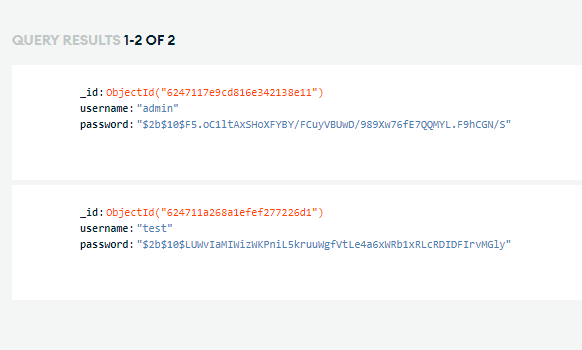
\includegraphics[width=12truecm, height=7truecm]{images/kollekcio.png}
	\caption{A felhasználói fiókokat tartalmazó kollekció}
	\label{fig:kollekcio}
\end{figure}

\noindent{\textbf{\large{Felhasználó hozááadása}}}\\

Első lépésként az \textit{adminadd.ejs} fájlban létrehozzunk a megfelelő űrlapot, az \texttt{action} paraméterét pedig \textit{post}-ra állítjuk. Az űrlap tartalma:

\begin{itemize}
\item{\textbf{Felhasználónév}: Egy text típusú \texttt{<input>} mező, ide kerül a hozzáadandó felhasználó neve.}
\item{\textbf{Jelszó}: Password típusú \texttt{<input>} mező, ez a leendő felhasználó jelszavát tartalmazza.}
\item{\textbf{Jelszó újra}: Password típusú \texttt{<input>} mező, a jelszó helyes bevitele miatt van szükség erre.}
\item{\textbf{Hozzáadás}: Egy \texttt{submit} típusú input-gomb, a kitöltött űrlapot ennek segítségével tudjuk elküldeni a szervernek.}
\end{itemize}

Elküldés után az applikációban kezelhetjük a felhasználói fiók hozzáadásának folyamatát.

Itt először különböző változókban eltároljuk a felhasználó által bevitt adatokat: a felhasználónevet, a jelszót, valamint az újbóli jelszóbevitelt. Ezután ellenőrzést hajtunk végre a jelszó mezőkön. Ha nem egyeznek, az adminisztrátor \textit{"A jelszavak nem egyeznek!"} hibaüzenetet kapja meg, majd vissza kell lépnie. Egyezés esetén csatlakozunk az adatbázishoz, és egy \texttt{findOne()} lekérdezésen keresztül megvizsgáljuk, hogy létezik-e az adott névvel felhasználói fiók. Ezzel lezárjuk az első lekérdezést. Ha létezik, szintén hibaüzenet kerül megjelenítésre ("\textit{Már létezik ilyen felhasználói fiók!}"). Ha nem létezik, elindítjuk a második lekérdezést, mely viszont már \texttt{insertOne()} típusú, ugyanis ezzel tudjuk beilleszteni a dokumentumba a felhasználói fiókot. Ezután a sikeres fiók-hozzáadásról üzenetet kapunk, majd visszalépünk az adminisztrációs felületre.\\

\noindent{\textbf{\large{Felhasználó módosítása}}}\\

Az előző metódushoz hasonlóan először az adatbeviteli felületet hozzuk létre (\textit{adminmodify.ejs}). Ugyanazokat a beviteli mezőket tartalmazza, mint a fiók hozzáadása, viszont az itt található mezők azonosítója más, a megkülönböztethetőség végett (Például a hozzáadás folyamatában a felhasználónevet tartalmazó mező azonosítója \texttt{addUName}, míg a módosítás űrlapjában található felhasználónév-mező azonosítója \texttt{modifyUName}).

Adatfeltöltés, és elküldés után az alkalmazásban folytatjuk a kezelést.

Változókban eltároljuk a felhasználó által beírt adatokat. Az első lépés itt is a jelszavak egyezőségének ellenőrzése. Ha nem egyeznek, hibaüzenetet küldünk. Ha egyeznek, inicializáljuk az első csatlakozást a szerverhez, aholis a felhasználónév meglétét ellenőrizzük. Ha nem létezik, hibaüzenetet küldünk, mivel csak meglévő felhasználói fiókot tudunk módosítani. Amennyiben létezik, egy \texttt{updateOne()} típusú lekérdezéssel módosítjuk a felhasználói fiók adatait. Visszajelzést küldünk a sikeres módosításról, majd visszalépünk az oldalra.\\

\noindent{\textbf{\large{Felhasználó eltávolítása}}}\\

Itt már csak egy felhasználónévre (és természetesen a \textit{Törlés} gombra) lesz szükségünk, hiszen a név alapján egyértelműen meghatározható, melyik fiókot szeretnénk eltávolítani a dokumentumból. Így az \textit{adminremove.ejs}-ben található űrlap csak a felhasználónévhez szükséges \texttt{<input>} mezőt, valamint az elküldést intéző gombot tartalmazza.

A következő lépés már ismert. Felhasználói adatbevitel, madj pedig elküldés. Továbbiakban az applikáció foglalkozik a metódussal.

A törlendő felhasználói fiók nevének változóban történő eltárolása után csatlakozunk az adatbázishoz, majd \texttt{findOne()} típusú lekérdezéssel rákeresünk a felhasználónévre. Ha a keresés nem járt sikerrel, hibaüzenet jelenik meg. Találat esetén egy új csatlakozást kezdeményezünk, ahol már \texttt{deleteOne()} típusú lekérdezés segítségével töröljük az adott névhez tartozó felhasználói fiókot. Sikeres adattörlés esetén visszajelzést küldünk az adminisztrátornak, majd visszalépünk.

%%%%%%%%%%%%%%%%%%%%%%%%%%%%%%%%%%%%%%%%%%%%%%% 4 . 3 . 4 %%%%%%%%%%%%%%%%%%%%%%%%%%%%%%%%%%%%%%%%%%%%%%%

\subsection{Fájlfeltöltés}

A következőekben a fájlok feltöltésének kezelését részletezzük. Az eddigiekhez hasonlóan - tekintettel arra, hogy ez a művelet is adatot oszt meg a szerverrel - ez a metódus is \texttt{post} típusú.\\

\noindent{\textbf{\large{Fájl feltöltése}}}\\

A folyamat a \textit{/fileupload} oldalon zajlik. Első körben a \textit{formidable} modul segítségével letároljuk a beérkező űrlapot, mely tartalmazza a feltöltendő fájlt. Ezután a modul \texttt{parse()} metódusát vesszük igénybe, ezzel értelmezzük és dolgozzuk fel az űrlap tartalmát. Alapvető hibaellenőrzést végzünk: Amennyiben a fájl neve megegyezik az üres string-gel (nincs fájlnév, azaz nincs kiválasztott fájl), úgy hibaüzenetet küldünk a felhasználónak (\textit{Nincs kiválasztott fájl!}). Ellenkező esetben először változókban eltároljuk:
\begin{itemize}
\item{a fájl(ok) feltöltésének mappáját (\textit{./views/files/uploads/}), a leendő fájlnévvel és kiterjesztésével együtt (a feltöltési útvonalat a \textit{path} modul segítségével hozzuk létre),}
\item{az eredeti fájl elérési útvonalát, és}
\item{az eredeti fájl tartalmát az \textit{fs} fájlkezelő modul \texttt{readFileSync()} függvénye segítségével.}
\end{itemize}
Következő lépésben szintén az \textit{fs} modul lesz hasznunkra, most a \texttt{existsSync()} metódust hívjuk meg, ennek segítségével a fájlok feltöltésének mappáját vizsgáljuk, azt keresve, hogy van-e a mappában azonos nevű fájl. Ha létezik ilyen, megakadályozzuk a feltöltést, és hibaüzenetet küldünk (\textit{Már létezik ilyen nevű fájl!}), így kiszűrve az azonos nevű fájlok feltöltésének problémáját. Viszont ha nem létezik, szabad az út a feltöltéshez. Még egyszer az \textit{fs} modult hívjuk segítségül, majd a \texttt{writeFile()} funkcióját meghívva a változóban korábban már eltárolt feltöltési útvonalra kiírunk egy új fájlt, és feltöltjük az eredeti fájl \texttt{readFileSync()} által feldolgozott tartalmával.\\

\noindent{\textbf{\large{Program feltöltése}}}\\

Ez a metódusa \textit{/programmeupload} oldalon történik, viszont a feltöltés kezelése szinte azonos a fájlfeltöltéssel. Az űrlap tartalmának változóban történő letárolása után a kiválasztott fájl ellenőrzését vizsgáljuk. Ha van kiválasztott fájl az űrlapban, letároljuk a fájlfeltöltéshez hasonlóan 3 változóban a feltöltés helyét (\textit{./views/programmes/uploads/}), fájlnévvel és kiterjesztéssel együtt, az eredeti elérési útvonalat, valamint az eredeti fájl tartalmát. Keresünk a mappában azonos nevű fájlt. Ha egyedi a fájlnév, akkor az eredeti fájl tartalmát kimásoljuk az általunk létrehozott, új fájlba, majd a sikeres feltöltő művelet után visszajelzést küldünk.

%%%%%%%%%%%%%%%%%%%%%%%%%%%%%%%%%%%%%%%%%%%%%%% 4 . 3 . 5 %%%%%%%%%%%%%%%%%%%%%%%%%%%%%%%%%%%%%%%%%%%%%%%

\subsection{Címek}

Az alkalmazás eddigi részében kizárólag \texttt{post} metódust használtunk az \textit{Express} modullal, ezután viszont csak \texttt{get}-re lesz szükségünk, mivel ezekben a kérésekben a szerverről kérünk le adatot. További jellemzői közé tartozik még, hogy a \texttt{post}-tal ellentétben ezek az oldalak könyvjelzőként menthetőek, valamint újratöltésükkor nem ütközünk problémába (\texttt{post} kérés újratöltése esetén az adatok újra elküldésre kerülnek, például \textbf{netbankon belüli tranzakciós kérés oldalának újratöltése esetén a tranzakció megismétlődik}, ezt kiküszöbölendő a böngésző értesítést küld ilyen esetben). Továbbá a küldés paraméterei megjelennek a böngésző címében, illetve mentésre kerülnek a böngésző előzményei közt. Ebből kifolyólag érzékeny adat továbbításakor nem érdemes ezt a metódust használni!

A címeket funkciójuk alapján különböző csoportokba osztjuk:

\begin{itemize}
\item{bejelentkezési oldal}
\item{felhasználói felület oldalai}
\item{adminisztrációs felület oldalai}
\item{sikerességet visszajelző oldalak}
\item{hibát jelző oldalak}
\end{itemize}

\noindent{\textbf{\large{Bejelentkezési oldal}}}\\

Ide egyetlen oldal tartozik, a bejelentkezési oldal, mely egyben az URL gyökerét is jelzi (vagyis, domain név betöltése esetén ez jelenik meg). Elérési útvonala "\textit{/}". Ezen az oldalon tudnak a felhasználók (és az adminisztrátor) bejelenkezni a megfelelő oldalra (a felhasználók a \textit{home} nevű főoldalra, az adminisztrátor pedig az \textit{/adminadd} oldalra), valamint a munkamenet lejáratát követően is erre az oldalra navigálhatnak.\\

\noindent{\textbf{\large{Felhasználói felület oldalai}}}\\

Ide soroljuk azokat az oldalakat, melyek között a (bejelentkezett) felhasználók navigálni tudnak. Amint azt már korábbi fejezetekben részleteztük, a felhasználók képesek lesznek:

\begin{itemize}
\item{böngészni fájlok között}
\item{letölteni fájlokat, programokat, illetve}
\item{feltölteni saját tartalmat.}
\end{itemize}

Ezen lehetőségeket szemlélteti az alábbi use-case diagram (\ref{fig:userusecase}. ábra):

\begin{figure}[h]
	\centering
		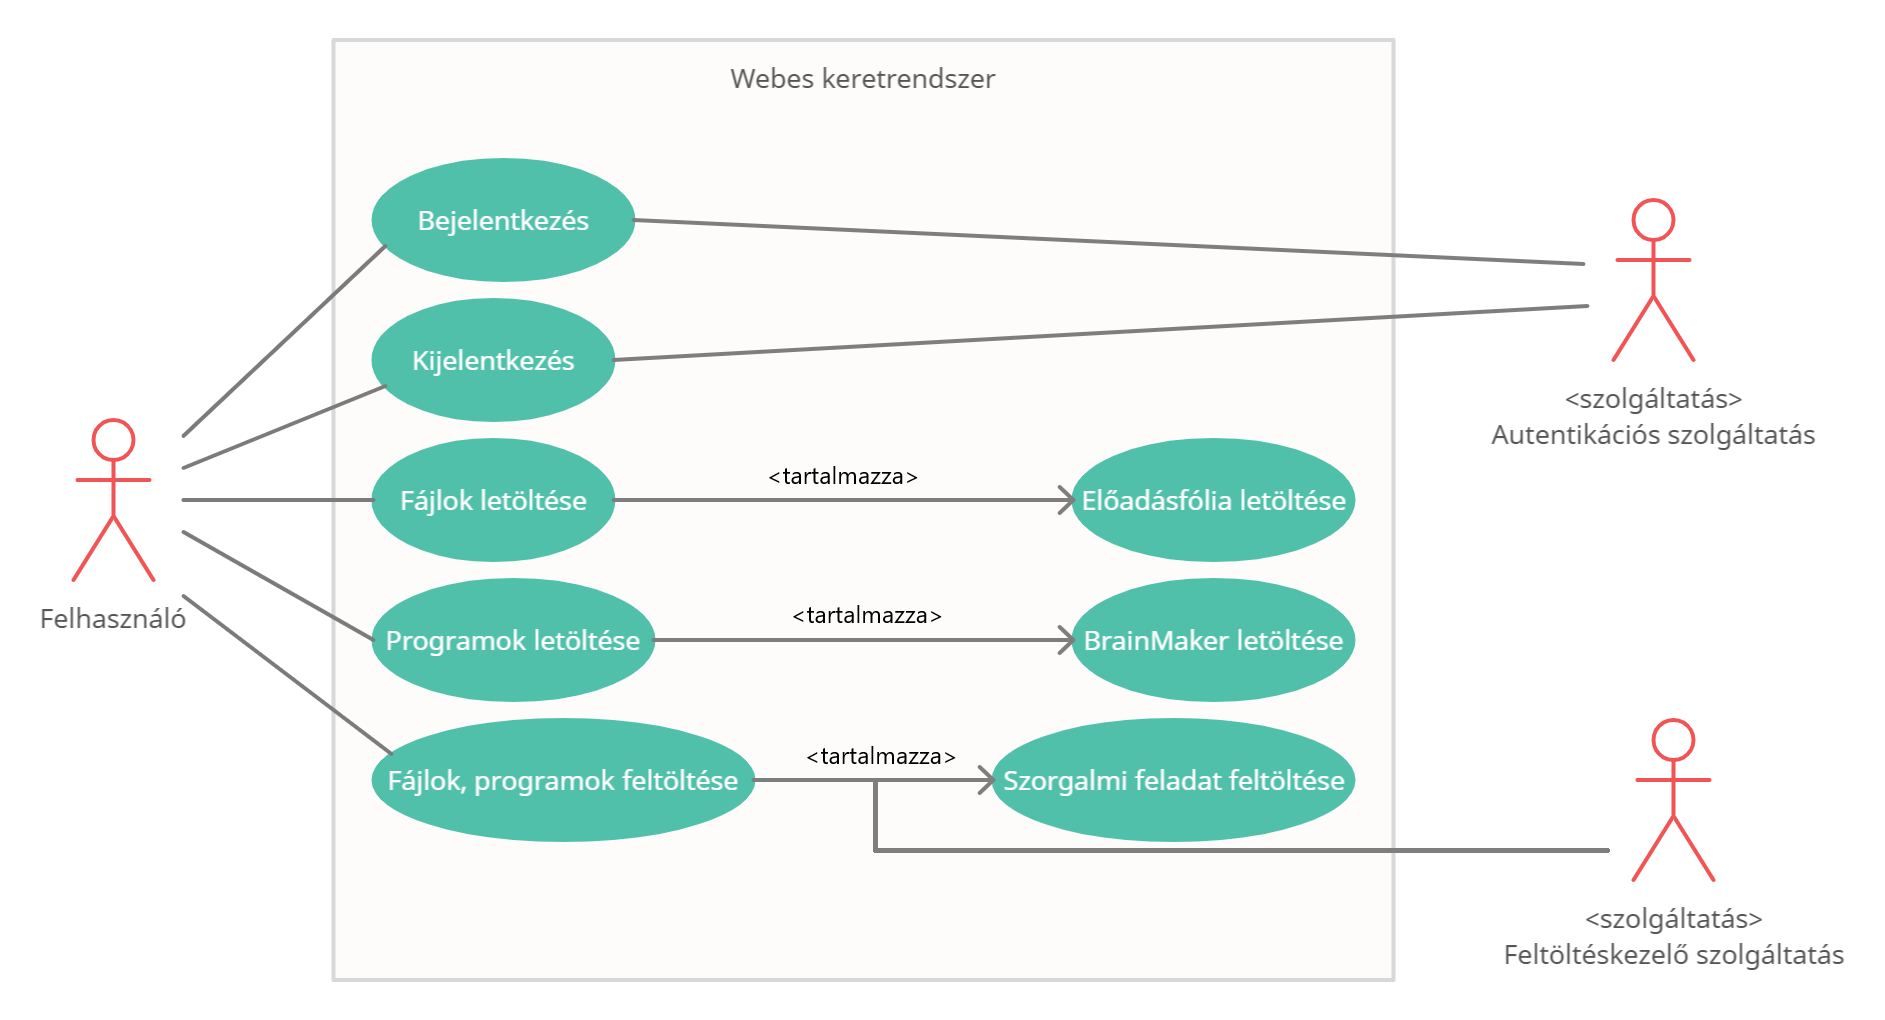
\includegraphics[width=15truecm, height=10truecm]{images/felhasznalo_use_case.png}
	\caption{A felhasználói felület}
	\label{fig:userusecase}
\end{figure}

A navigációt a weboldal felső részében található zöld menü segítségével végezhetik a felhasználók. A menü felett jelenik meg annak az oldalnak a neve, melyen a felhasználó éppen tartózkodik. A \textit{mainStyle.css} nevű CSS stíluslap adja ezen oldalak kinézetét, mely szerint a kurzor menüpontokra való húzása (\texttt{hover}) esetén a kijelölt menüpont szürke kiemelő színt kap, így megkülönböztetve a menüpontokat. A \textit{Fájlok}, valamint a \textit{Programok} menüpontok \textit{hover} eseménye esetén legördülnek, és két almenüpont válik előrhetővé számunkra: a \textit{Fájlok} menüpontból a \textit{Tananyagok} és a \textit{Feltöltés}, a \textit{Programok} menüpontból pedig a \textit{Demonstrációk} és a \textit{Feltöltés} almenüpontok jelennek meg. Az almenüpontok háttérszíne fekete, kijelőlés esetén viszont ugyanazt a szürkés árnyalatot kapják, mint a főmenüpontok. Kattintás hatására pedig a tényleges navigáció zajlik le. Attól függően, hogy melyik menüpontra kattintottunk, a navigáció változatos lehet:

\begin{itemize}
\item{\textbf{Főoldal}: Navigáció a "\textit{/home}" oldalra.}
\item{\textbf{Fájlok/Tananyagok}: Navigáció a "\textit{/files}" oldalra.}
\item{\textbf{Fájlok/Feltöltés}: Navigáció a "\textit{/fileupload}" oldalra.}
\item{\textbf{Programok/Demonstrációk}: Navigáció a "\textit{/programmes}" oldalra.}
\item{\textbf{Programok/Feltöltés}: Navigáció a "\textit{/programmeupload}" oldalra.}
\end{itemize}

\noindent{\textbf{\large{Adminisztrációs felület oldalai}}}\\

Ide azokat az oldalakat soroljuk, melyek között az adminisztrátor böngészni tud. Ezen oldalakon az adminisztrátornak lehetősége van felhasználót hozzáadni, felhasználó meglévő adatait módosítani, valamint felhasználói fiókot törölni.

A megfelelő felhasználóba való bejelentkezés után a program automatikusan az adminisztrátori felületbe továbbít minket. Az itt rendelkezésünkre álló lehetőségeket szemlélteti az alább található use-case diagram (\ref{fig:adminusecase}. ábra):

\begin{figure}[h]
	\centering
		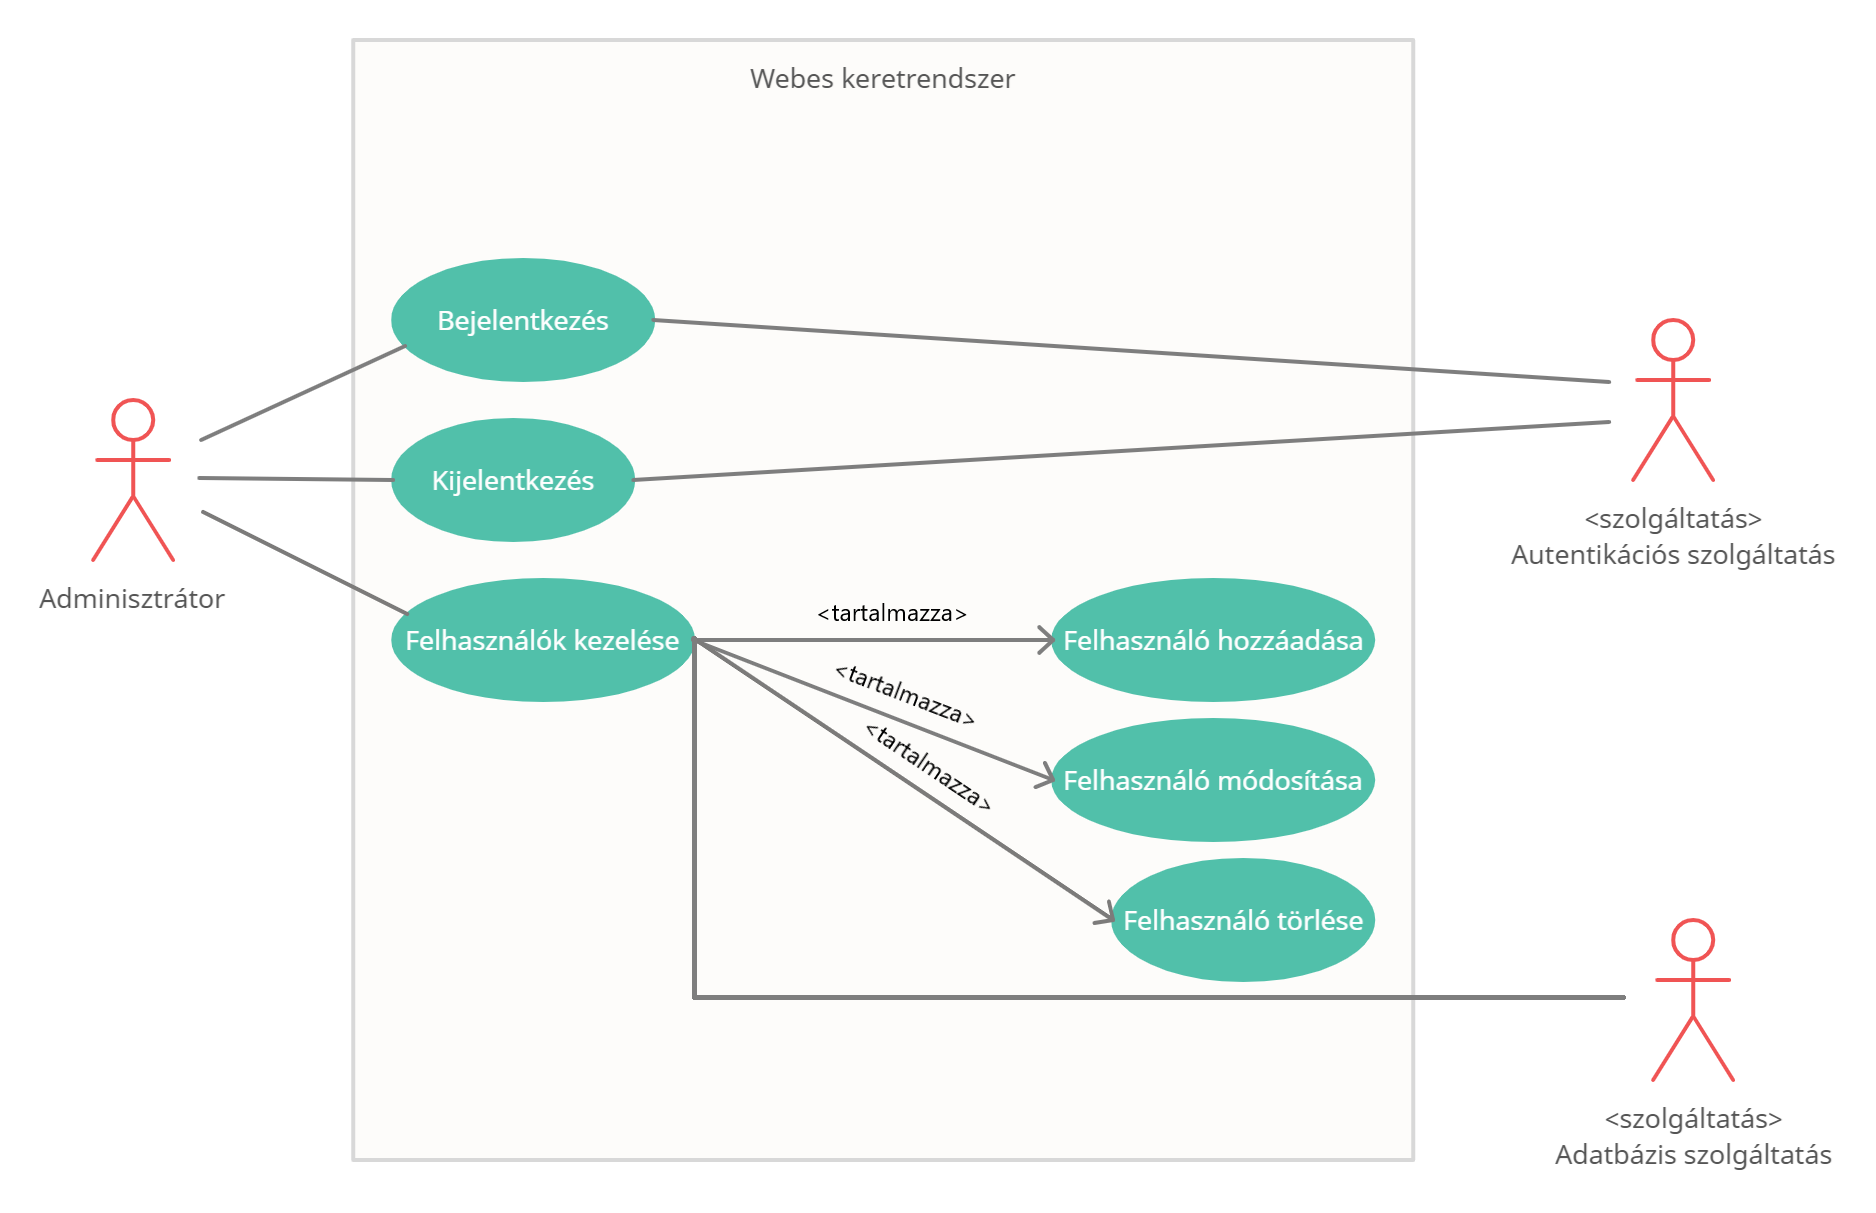
\includegraphics[width=15truecm, height=10truecm]{images/adminisztrator_use_case.png}
	\caption{Az adminisztrátori felület}
	\label{fig:adminusecase}
\end{figure}

\newpage

A felület stílusa megegyezik a felhasználói felület stílusával, mivel ezen oldalak is a \textit{mainStyle.css} stíluslapot használják. A főmenüpontok zöldek, a jelenlegi oldalt jelző cím szürke, menüpont kijeöléskor pedig szürke hátteret kapnak. Itt nincsenek almenüpontok, csak három főmenüpont:

\begin{itemize}
\item{\textbf{Felhasználó hozzáadása}: Navigáció az "\textit{/adminadd}" oldalra.}
\item{\textbf{Felhasználó módosítása}: Navigáció az "\textit{/adminmodify}" oldalra.}
\item{\textbf{Felhasználó törlése}: Navigáció az "\textit{/adminremove}" oldalra.}
\end{itemize}

\noindent{\textbf{\large{Sikerességet visszajelző oldalak}}}\\

Ide tartoznak azok az oldalak, melyek a sikeres műveletek (például adatbázis sikeres frissítése) után kerülnek megjelenítésre. Ezek mindegyike a \textit{successStyle.css} nevű stíluslapot veszi igénybe. Ebbe a kategóriába soroljuk:

\begin{itemize}
\item{\textbf{Adatbázis sikeres frissítése}: Navigáció a "\textit{/dbsuccess}" oldalra. Ide az adminisztrátor oldalán található \textit{Felhasználó hozzáadása}, \textit{/Felhasználó módosítása}, valamint a \textit{/Felhasználó törlése} műveletek sikeres elvégzése után jutunk el.}
\item{\textbf{Feltöltés sikeres}: Navigáció az "\textit{/uploadsuccess}" oldalra. A \textit{/fileupload}, illetve a \textit{/programmeupload} oldalakon elvégezhető feltöltés (végbement, sikeres) művelete után jelenik meg a felhasználók számára ez az oldal.}
\end{itemize}

\noindent{\textbf{\large{Hibajelző oldalak}}}\\

Ebbe a csoportba tartoznak azok az oldalak, melyek a hibás műveleteket jelzik vissza, vagy elkerülendő problémák miatt van szükség rájuk. Ezen oldalak megjelenése a \textit{/errorStyle.css} stíluslap alapján történik. Ide tartoznak:

\begin{itemize}
\item{\textbf{Helytelen jelszó}: Navigáció a "\textit{/badauth}" oldalra. Ezt akkor jelenítjük meg, ha a felhasználó, vagy az adminisztrátor nem a fióknévhez kapcsolt jelszót gépeli be a jelszó mezőbe.}
\item{\textbf{Már létező fájl}: Navigáció a "\textit{/fileexists}" oldalra. Ezzel a hibaüzenettel találkozunk abban az esetben, "\textit{Fájlok/Feltöltés}", vagy a "\textit{Programok/Feltöltés}" menüpont alatt olyan állományt szeretnénk feltölteni, melynek neve már megtalálható a megfelelő "\textit{files/uploads}", vagy "\textit{programmes/uploads}" mappában (tehát már feltöltésre került azonos nevű fájl).}
\item{\textbf{Helytelen vagy lejárt munkamenet}: Navigáció a "\textit{/invalid}" oldalra. Akkor szembesülünk ezzel az üzenettel, ha a bejelentkezéstől számított 30 perces munkamenet lejár, és az idő lejárta után próbálunk meg műveleteket végezni az oldalon (például másik oldal betöltése a menün keresztül). Továbbá, amennyiben a címsorból próbáljuk meg elérni az oldalakat, szintén ezzel a hibával találkozunk. Érdemes lehet megjegyezni, hogy míg a többi hibajelző oldalon "\textit{Vissza}" gomb található, mely a böngésző előzménye alapján vezet vissza az előző meglátogatott oldalra a \texttt{history.back()} paranccsal, addig ezen az oldalon egy "\textit{Bejelentkezés}" gomb található, mely visszairányítja a böngészőt a \texttt{window.location} paraméter változtatásával a bejelentkezési felületre.}
\item{\textbf{Nincs kiválasztott fájl}: Navigáció a "\textit{/nofile}" oldalra. Amikor a felhasználó úgy küldi el a "\textit{Fájlok/Feltöltés}", vagy a "\textit{Programok/Feltöltés}" oldalon található űrlapot, hogy nem választott ki fájlt, akkor ez a hibaüzenet jelenik meg számunkra.}
\item{\textbf{Jogosulatlan felhasználó}: Navigáció a "\textit{/notadmin}" oldalra. Erre akkor van szükség, ha egy nem-adminisztrátor szeretne hozzáférni (címsor segítségével) az adminisztrátori felülethez.}
\item{\textbf{Nincs ilyen felhasználó}: Navigáció a "\textit{/notfound}" oldalra. A bejelentkezési oldalról kaphatunk ilyen hibajelzést. Az autentikáció során a felhasználó által begépelt név alapján keresünk felhasználói fiókot az adatbázisban. Ha nem találtunk egyet sem (nincs ilyen névvel felhasználói fiók), akkor erre az oldalra irányít minket az applikáció.}
\item{\textbf{Nem egyező jelszavak}: Navigáció a "\textit{/notmatching}" oldalra. Ezt a hibaüzenetet két oldalról is kaphatjuk: az egyik a \textit{Felhasználó hozzáadása}, a másik pedig a \textit{Felhasználó módosítása} nevű, adminisztrátori felületen fellelhető oldal. Értelemszerűen mindkét oldalon ugyanaz a hiba váltja ki ennek a hibaüzenetnek a megjelenítését: Ha az adminisztrátor nem ugyanazt a jelszót gépeli be a két \textit{Jelszó} mezőbe.}
\item{\textbf{Már létező felhasználó}: Navigáció a "\textit{/userexists}" oldalra. Ez az adminisztrátor számára megjelenő üzenet. Akkor következik be ez a hiba, ha olyan felhasználói fiókot próbál hozzáadni az adatbázishoz, melynek neve már szerepel az adatbázisban. Könnyű belátni, hogy két azonos nevű felhasználó nem szerepelhet a fiókok nyilvántartásában.}
\end{itemize}

%%%%%%%%%%%%%%%%%%%%%%%%%%%%%%%%%%%%%%%%%%%%%%% 4 . 3 . 6 %%%%%%%%%%%%%%%%%%%%%%%%%%%%%%%%%%%%%%%%%%%%%%%

\subsection{A hallgatói felület}

A hallgatói felület eléréséhez először a login oldalon való bejelentkezés szükségeltetik. Így tehát a felület elérése előtt elsőkörben a bejelentkezési felülettel találkoznak a hallgatók/felhasználók (\ref{fig:login}. ábra). 

\begin{figure}[h]
	\centering
		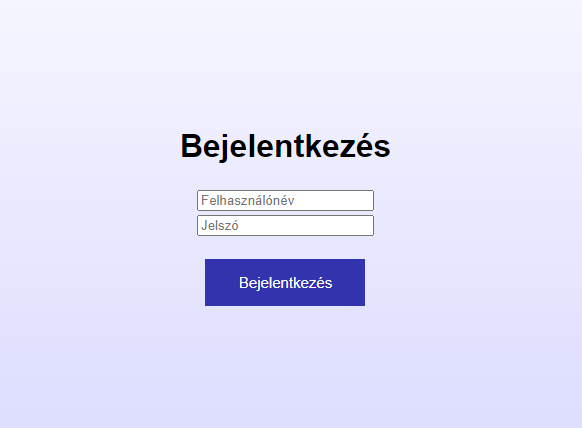
\includegraphics[width=10truecm, height=7truecm]{images/bejelentkezes.png}
	\caption{A bejelentkezési felület}
	\label{fig:login}
\end{figure}

\newpage

Sikertelen bejelentkezés esetén hibaüzenettel szembesülünk. Ezt okozhatja az, hogy a felhasználónév nem található az adatbázisban, vagy az, hogy a névhez tartozó jelszó nem megfelelő. Sikeres bejelentkezési folyamat esetén viszont a hallgatói főoldalon találjuk magunkat (\ref{fig:homeMenu}. ábra).

\begin{figure}[h]
	\centering
		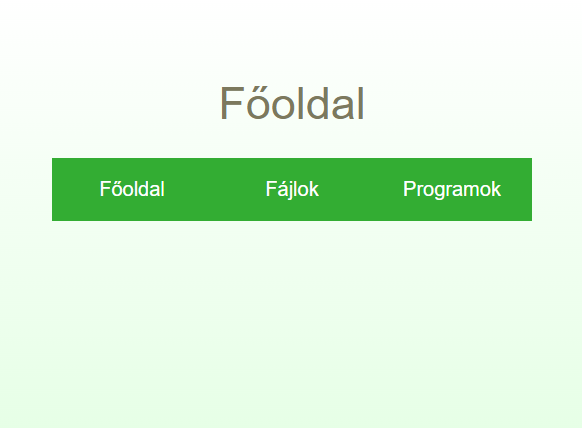
\includegraphics[width=10truecm, height=7truecm]{images/fooldal.png}
	\caption{A főoldal menüje}
	\label{fig:homeMenu}
\end{figure}

Fontos megjegyezni, hogy a munkafolyamat a bejelentkezés pillanatától számított 30 perc múlva kiléptet, és újabb bejelentkezési folyamat után enged vissza (\ref{fig:invalid}. ábra). Továbbá, a \textit{Kijelentkezés} gombra kattintva - azon kívül, hogy átirányít a bejelentkezési felületre - véget ér a munkafolyamat.

\begin{figure}[h]
	\centering
		
\includegraphics[width=10truecm, height=7truecm]{images/lejart_munkamenet.png}
	\caption{A munkamenet lejáratát jelző hibaüzenet}
	\label{fig:invalid}
\end{figure}

A főoldalon a legördülő menü lesz a felhasználók segítségére, ugyanis ezen keresztül történik a navigáció, melyet a korábbi fejezetekben részleteztünk. Maga a menü egyszerű, gombokból (\texttt{<button>}-okból) áll, melyeket stíluslapok segítségével kényelmesebbé, esztétikusabbá alakítunk.

Annak érdekében, hogy egyéb fontos információt meg tudjunk jeleníteni, létrehoztunk egy "\textit{sidebar}"-t. Ez nem más, mint a weboldalak bal oldalán elhelyezkedő oszlop, melyet adattárolásra rendszeresítettünk. Ennek szélessége mindig az adott képernyő méretéhez igazodik, pontosan a képernyő-szélesség 12\%-át foglalja el. Ennek megvalósítása egy egyszerű táblázattal történt. A menü alatt egy "láthatatlan" táblázatot hoztunk létre (egy olyan táblázatot, melynek 0 képpontnyi vastag szegélye van, így ugyan van szegélye, de nem látható). Ennek a táblázatnak két cellája van. A bal oldali cella szolgáltatja a már említett sidebar-t. A jobb oldali cella tölti ki a képernyő-szélesség maradékát, melyben a menüpontok szerinti tartalmat jelenítjük meg.

Mindezen felül a képernyő jobb felső sarkában található a \textit{Kijelentkezés} gomb, melynek segítségével visszatérhetünk a bejelentkezési oldalra. Értelemszerűen a kijelentkezés folyamata után a munkamenetünk véget ér, így ha vissza szeretnénk térni a felhasználói felületre, újabb bejelentkezésre lesz szükségünk.

%%%%%%%%%%%%%%%%%%%%%%%%%%%%%%%%%%%%%%%%%%%%%%% 4 . 3 . 7 %%%%%%%%%%%%%%%%%%%%%%%%%%%%%%%%%%%%%%%%%%%%%%%

\subsection{Az adminisztrátori felület}

A login oldalon a megfelelő (adminisztrátori) felhasználóba való bejelentkezés után a program automatikusan az adminisztrátori felületbe továbbít minket (\ref{fig:admin}. ábra).

\begin{figure}[h]
	\centering
		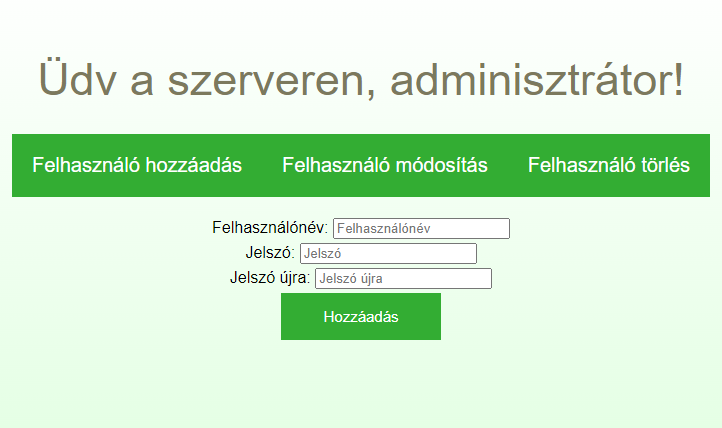
\includegraphics[width=12truecm, height=7truecm]{images/admin_oldal.png}
	\caption{Az adminisztrátori felület}
	\label{fig:admin}
\end{figure}

Amennyiben illetéktelenül próbálkozunk hozzáférni ehhez a felülethez (tehát, ha hallgatói fiókba jelentkezünk be, vagy ha egyáltalán nem jelentkezünk be), úgy hibaüzenet fogad minket (\ref{fig:nemadmin}. ábra)

\begin{figure}[h]
	\centering
		
\includegraphics[width=10truecm, height=7truecm]{images/nemadmin.png}
	\caption{Illetéktelen felhasználó esetén megjelenő hibaüzenet}
	\label{fig:nemadmin}
\end{figure}

\newpage

Ellenkező esetben (adminisztrátori fiókba való bejelentkezéskor) a rendszer átirányít a "\textit{Felhasználó hozzáadása}" (\textit{/adminadd}) oldalra. Ez a felület hasonló a hallgatói felülethez, hiszen ugyanazt a stíluslapot (\textit{mainStyle.css}) használja. Itt is megtalálható egy menü, azonban itt nem ugyanazok a menüpontok találhatóak:

\begin{itemize}
\item{\textbf{Felhasználó hozzáadása}: Ezezn az oldalon lehet új felhasználói fiókot hozzáadni az adatbázishoz.}
\item{\textbf{Felhasználó módosítása}: Itt lehet egy felhasználó már meglévő fiókjának jelszavát módosítani.}
\item{\textbf{Felhasználó törlése}: Itt pedig egy meglévő felhasználói fiókot lehet a neve alapján törölni az adatbázisból.}
\end{itemize}

Az előző alfejezetben ismertetett \textit{sidebar}, valamint a \textit{Kijelentkezés} gomb itt is megtalálható.

Érdemes megjegyezni azt a tényt, hogy munkamenet szempontjából az adminisztrátort is felhasználóként kezeljük! Ez azt jelenti, hogy a bejelentkezéstől számított 30 perc után az adminisztrátort is kijelentkezteti a program, és újra be kell jelentkeznie.